\documentclass[tikz,border=6pt]{standalone}

\usepackage{tikz}
\usetikzlibrary{arrows.meta,backgrounds,fit,positioning}

\definecolor{StepBlue}{RGB}{92,140,214}
\definecolor{StepTeal}{RGB}{82,176,164}
\definecolor{StepOrange}{RGB}{243,156,18}
\definecolor{StepPurple}{RGB}{155,89,182}
\definecolor{StepGreen}{RGB}{93,173,110}
\definecolor{StepRed}{RGB}{214,96,96}
\definecolor{LaneGray}{RGB}{243,245,247}

\tikzset{
  stepbox/.style={
    draw,
    rounded corners=3pt,
    thick,
    align=center,
    minimum width=3.1cm,
    minimum height=1.08cm,
    fill=white,
    font=\small
  },
  arrow/.style={-Latex,thick},
  lane/.style={draw,rounded corners=6pt,fill=LaneGray,inner sep=8pt},
  lanetitle/.style={font=\footnotesize\bfseries}
}

\begin{document}
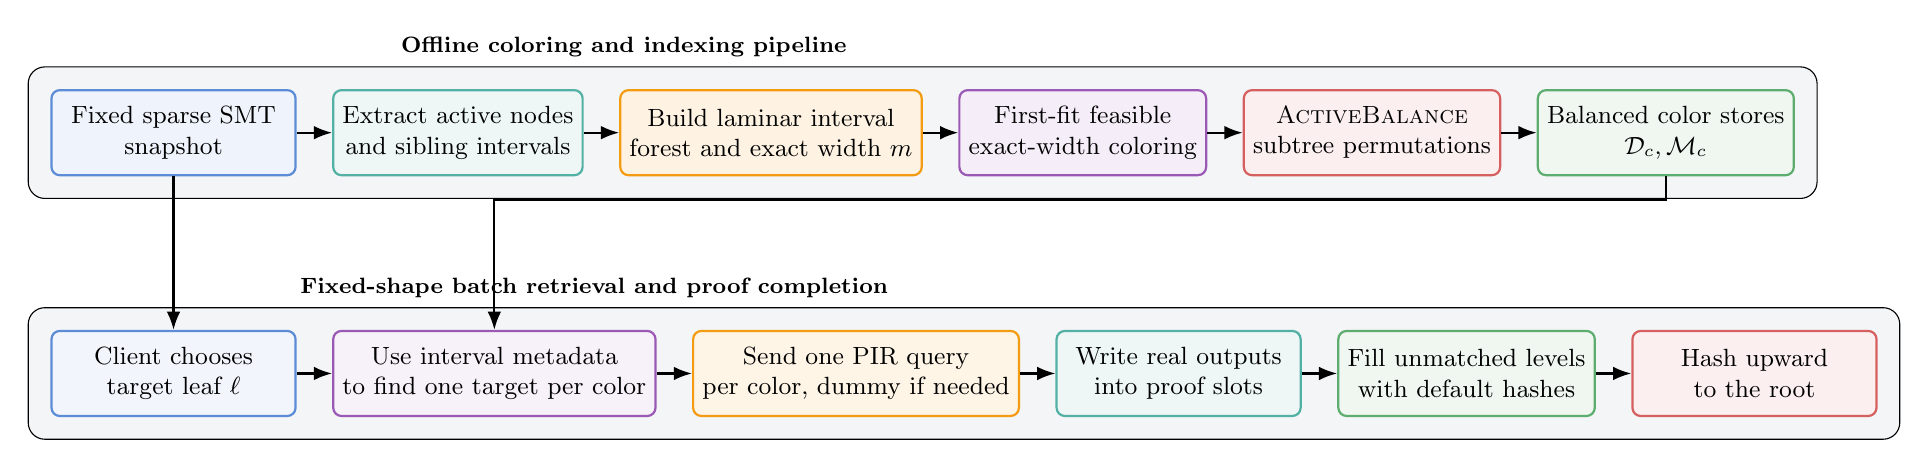
\begin{tikzpicture}[node distance=0.55cm and 0.45cm]

\node[stepbox,draw=StepBlue,fill=StepBlue!10] (o1)
  {Fixed sparse SMT\\snapshot};
\node[stepbox,draw=StepTeal,fill=StepTeal!10,right=of o1] (o2)
  {Extract active nodes\\and sibling intervals};
\node[stepbox,draw=StepOrange,fill=StepOrange!12,right=of o2] (o3)
  {Build laminar interval\\forest and exact width $m$};
\node[stepbox,draw=StepPurple,fill=StepPurple!10,right=of o3] (o4)
  {First-fit feasible\\exact-width coloring};
\node[stepbox,draw=StepRed,fill=StepRed!10,right=of o4] (o5)
  {\textsc{ActiveBalance}\\subtree permutations};
\node[stepbox,draw=StepGreen,fill=StepGreen!10,right=of o5] (o6)
  {Balanced color stores\\$\mathcal{D}_c,\mathcal{M}_c$};

\node[stepbox,draw=StepBlue,fill=StepBlue!8,below=1.95cm of o1] (q1)
  {Client chooses\\target leaf $\ell$};
\node[stepbox,draw=StepPurple,fill=StepPurple!8,right=of q1] (q2)
  {Use interval metadata\\to find one target per color};
\node[stepbox,draw=StepOrange,fill=StepOrange!10,right=of q2] (q3)
  {Send one PIR query\\per color, dummy if needed};
\node[stepbox,draw=StepTeal,fill=StepTeal!10,right=of q3] (q4)
  {Write real outputs\\into proof slots};
\node[stepbox,draw=StepGreen,fill=StepGreen!10,right=of q4] (q5)
  {Fill unmatched levels\\with default hashes};
\node[stepbox,draw=StepRed,fill=StepRed!10,right=of q5] (q6)
  {Hash upward\\to the root};

\draw[arrow] (o1) -- (o2);
\draw[arrow] (o2) -- (o3);
\draw[arrow] (o3) -- (o4);
\draw[arrow] (o4) -- (o5);
\draw[arrow] (o5) -- (o6);

\draw[arrow] (q1) -- (q2);
\draw[arrow] (q2) -- (q3);
\draw[arrow] (q3) -- (q4);
\draw[arrow] (q4) -- (q5);
\draw[arrow] (q5) -- (q6);

\draw[arrow] (o1.south) -- ++(0,-0.30) -| (q1.north);
\draw[arrow] (o6.south) -- ++(0,-0.30) -| (q2.north);

\begin{pgfonlayer}{background}
  \node[lane,fit=(o1)(o6),label={[lanetitle]above left:{Offline coloring and indexing pipeline}}] {};
  \node[lane,fit=(q1)(q6),label={[lanetitle]above left:{Fixed-shape batch retrieval and proof completion}}] {};
\end{pgfonlayer}

\end{tikzpicture}
\end{document}
